\section{Zielsetzung}
\label{sec:Zielsetzung}
Ziel des Versuchs ist es die Aufspaltung der Energieniveaus durch den Zeeman-Effektes,
sowie der Hyperfeinstruktur auszumessen. Des Weiteren soll der Landé-Faktor des Gesamtdrehimpulses
des Atoms bestimmt werden. Ebenso soll das transidente Verhalten näher untersucht werden.

\section{Theorie}
\label{sec:Theorie}
\subsection{Atomaufbau}
\label{sec:atomaufbau}
Aus der Quantenmechanik ist bekannt, dass das Atom aus einem Kern und einer Atomhülle besteht.
In der Atomhülle bewegen sich die Elektronen auf festen Energieniveaus. Dabei sind die inneren
Niveaus voll besetzt. Die äußeren Niveaus sind nach der Boltzmann-Verteilung
\begin{equation}
  \label{eqn:boltz}
  \frac{N_2}{N_1} = \frac{g_2 \cdot \exp{\left(\sfrac{-W_2}{k_\text{B}T}\right)}}{g_1 \cdot \exp{\left(\sfrac{-W_1}{k_\text{B}T}\right)}}
\end{equation}
temperaturabhängig besetzt. Dabei bezeichnen die $N_\text{i}$ die Besetzungszahlen, $g_\text{i}$ den Entartungsgrade
der Energieniveaus $W_\text{i}$, wobei $W_2 > W_1$ gilt. Damit die Formel auch ihre Gültigkeit besitzt
muss sich das Atom bei Temperatur $T$ im thermischen Gleichgewicht befinden.
Um zwischen den Energieniveaus zu wechseln müssen Quanten der Energie
\begin{equation}
  \label{eqn:energiedifferenz}
  h \nu = W_2 - W_1
\end{equation}
emittiert oder absorbiert werden. 
In diesem Versuch werden Alkaliatome untersucht, diese zeichnen sich dadurch aus, dass sich nur ein 
Elektron auf dem äußersten Niveau befindet, was die Rechnungen deutlich vereinfacht.

\subsection{Magnetisches Moment der Atomhülle}
\label{sec:atomhülle}
Aus dem Bahndrehimpuls der Eektronen $\vec{L}$ und dem Spin der Elektronen $\vec{S}$ ergibt sich der
Gesamtdrehimpulses $\vec{J} = \vec{L} + \vec{S}$. Zu jedem Drehimpuls gehört auch ein magnetisches Moment.
Dabei ergibt sich das magnetische Moment für den Gesamtdrehimpuls 
\begin{equation*}
  \vec{\mu_\text{J}} = \vec{\mu_\text{L}} + \vec{\mu_\text{S}}
\end{equation*}
aus der Summe der magnetischen Momente für Spin 
\begin{equation}
\label{eqn:magspin}
  \vec{\mu_\text{S}} = -g_\text{S} \mu_\text{B} \vec{S}
\end{equation}
und Bahndrehimpuls
\begin{equation}
  \label{ean:magbahn}
  \vec{\mu_\text{L}} = - \mu_\text{B} \vec{L}.
\end{equation}
Mit dem Betrag eines jeden Drehimpulses $|\vec{L'}| = \sqrt{L' \left(L'+1\right)}$ und den
in Abbildung \ref{fig:magnmoment} dargestellten Zusammenhängen ergibt sich nach Anwenden des Kosinussatzes
und umstellen
\begin{equation}
  \label{eqn:gj}
  g_\text{J} = \frac{\num{3.0023}J(J+1)+\num{1.0023}[S(S+1)-L(L+1)]}{2J(J+1)},
\end{equation}
dabei wird $g_\text{S} = \num{2.00232}$ verwendet.
Wird nun ein äußeres Magnetfeld $\vec{B}$ angelegt, so spalten sich die Energieniveaus in $2J+1$ Unterniveaus auf.
Dies hat seine Ursache in der Wecheselwirkung des magnetischen Moments mit dem Magnetfeld und der Richtunsquantelung.
Bekanntlich präzidiert $\vec{\mu_\text{J}}$ um die Feldrichtung des äußeren magnetfeldes und der senkrtechte Anteil mittelt 
sich herraus. Für die $z$-Komponete ergibt sich mit der Richtungsquantelung die Wecheselwirkungsenergie zu
\begin{equation}
  \label{eqn:wwenergie}
  U_\text{magn} = M_\text{J} g_\text{J} \mu_\text{B} |\vec{B}|,
\end{equation}
mit der Orientierungsquantenzahl $M_\text{J} = -J, \ldots, J-1 ,J$. Dieser Effekt ist besser bekannt unter
dem Namen Zeeman-Effekt.
\begin{figure}
  \centering
  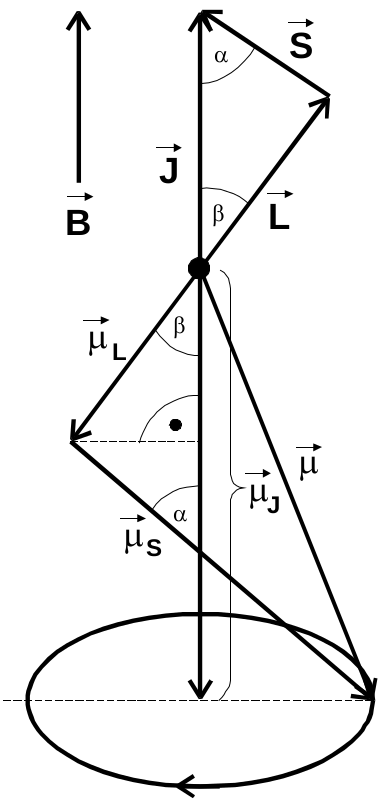
\includegraphics[height=5.5cm]{content/pictures/MagnMoment.png}
  \caption{Skizze zur Veranschaulichung der Zusammenhänge für die Bestimmung des magnetischen Moments der Elektronenhülle \cite{anleitung}.}
  \label{fig:magnmoment}
\end{figure}

\subsection{Magnetisches Moment des Atoms}
\label{sec:atom}
Neben den Hüllenelektronen trägt auch der Kern mit seinem Kernspin $I$ zum Gesamtdrehimpuls des Atoms $F$ bei.
Dabei verläuft dies analog zu Abschnitt \ref{sec:atomhülle}, genauer
\begin{equation*}
  \vec{F} = \vec{J} + \vec{I}.
\end{equation*}
Auf Grund der Kopplung vom Kernspin mit dem Gesamtdrehimpuls der Atomhülle ergibt sich die Aufspaltung der 
Hyperfeinstruktur, dabei darf das äußere Magnetfeld allerdings nicht zu stark sein.
Es ergeben sich $2J+1 (J<I)$ beziehungsweise $2I+1 (I<J)$  Unterniveaus. Dies Unterniveaus werden mit Hilfe
der Quantenzahl $F = |I-J|, \ldots,I+J-1, I+J$ unterschieden. Es spalten sich also zunächst die Feinstrukturniveaus
in die Hyperfeinstrukturniveaus auf, welche unter dem Einfluss eines äußeren Magnetfelds weiter in die 
Zeeman-Niveaus aufspalten. Die Energiedifferenz der Zeeman-Niveaus ergibt sich zu
\begin{equation}
  \label{eqn:zeeman}
  U_\text{Z} = g_\text{F} \mu_\text{B} |\vec{B}|.
\end{equation}
Mit Hilfe des magnetischen Moments des Atoms
\begin{equation*}
  \vec{\mu_\text{F}} = -g_\text{F} \mu_\text{B} \vec{F}
\end{equation*}
und der richtungsorientierten Addition der Beiträge der magnetischen Momente von Atomkern und Atomhülle
ergibt sich der Landé-Faktor
\begin{equation}
  \label{eqn:lande}
  g_\text{F} = g_\text{J} \frac{F(F+1)+J(J+1)-I(I+1)}{2F(F+1)}.
\end{equation}

\subsection{Optisches Pumpen}
\label{sec:pumpen}
Als optisches Pumpen wird eine Umbesetzung der thermischen Besetzung der Energieniveaus bezeichnet.
Um dieses Pumpen zu ermöglichen wird die in Abschnitt \ref{sec:atomhülle} beschriebene Zeeman-Aufspaltung benötigt.
Für ein Alkaliatome ergibt sich im Grundzustand ein $\ce{^2 S_{\sfrac{1}{2}}}$ Niveau, sowie die Niveaus
$\ce{^2 P_{\sfrac{1}{2}}}$ und $\ce{^2 P_{\sfrac{3}{2}}}$ für den ersten angeregten Zustand, wenn der
Kerndrehimpuls vernachlässigt wird. Abbildung \ref{fig:aufspaltung} zeigt die Zeeman-Aufspaltung in die Zeeman-Niveaus für
die beiden Zustände mit $J=\sfrac{1}{2}$, also den optischen $\text{D}_1$-Übergang. Unter zu Hilfe nahme der Auswahlregeln für erlaubte Übergänge
\begin{align*}
  \Delta L & = \pm 1 \\
  \Delta M_\text{J} & = 0, \pm 1
\end{align*}
\begin{figure}
  \centering
  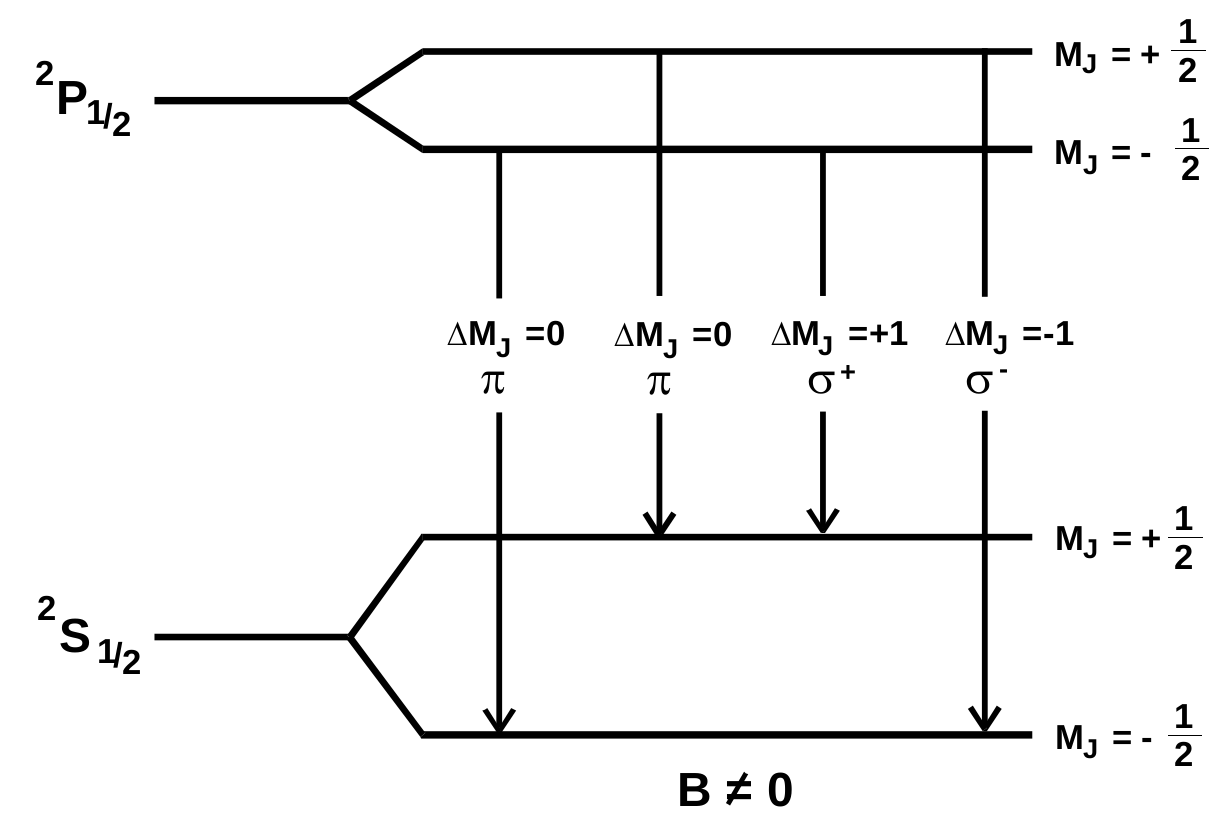
\includegraphics[height=8cm]{content/pictures/Energieniveaus.png}
  \caption{Die Energieniveau-Aufspaltung unter Einfluss eines $\vec{B}$-Feldes \cite{anleitung}.}
  \label{fig:aufspaltung}
\end{figure}
ergeben sich die in Abbildung \ref{fig:aufspaltung} als Pfeile eingezeichneten Übergänge.
Diese unterscheiden sich in Polarisation und Energie der ausgesendeten Quanten. So entspricht 
in Richtung von $\vec{B}$ ausgesendetes rechtszirkular-polarisiertes Licht dem $\sigma^+$-Übergang und 
linkszirkular-polarisiertes Licht dem $\sigma^-$-Übergang. Bei den $\pi$-Übergängen 
handelt es sich um emittiertes beziehungsweise absorbiertes Licht, welches linear-polarisiert
(parallel zu $\vec{B}$) ist und senkrecht zu $\vec{B}$ abgestrahlt wird.

Wird eine Dampfzelle bei der Temperatur $T$ mit einem Dampf aus Alkaliatomen befüllt und 
mit einem Magnetfeld durchsetzt, so befinden sich die Atome zunächst im Grundzustand. Nun wird rechtszirkular-polarisiertes
$\text{D}_1$-Licht eingestrahlt und damit der Übergang mit $\Delta M_\text{J} = +1$ ermöglicht. 
Dadurch werden die Elektronen aus dem $\ce{^2 S_{\sfrac{1}{2}}}$-Niveau mit $M_\text{J}=\sfrac{-1}{2}$ in das 
$\ce{^2 P_{\sfrac{1}{2}}}$-Niveau mit $M_\text{J}=\sfrac{1}{2}$ angehoben. Da es für die Emission
keine weiteren Einschränkungen gibt, finden beide Übergänge ins Grundniveau statt. Es werden aber immer nur
Elektronen aus dem Niveau mit $M_\text{J}=\sfrac{-1}{2}$ angeregt und da kein Übergang innerhalb eines 
Niveaus erlaubt ist, reichern sich die Elektronen im Niveau mit
$M_\text{J}=\sfrac{1}{2}$ an und das mit $M_\text{J}=\sfrac{-1}{2}$ wird entleert. Somit ergibt sich eine 
nicht nach \eqref{eqn:boltz} gegebene thermische Besetzung. 
Mit Hilfe einer Photozelle auf der anderen Seite der Zelle wir die Transparenz des Gases beobachtet.
Wird das $\ce{^2 S_{\sfrac{1}{2}}}$-Niveau ($M_\text{J}=\sfrac{1}{2}$) leer, so wird kein $\text{D}_1$-Licht
mehr absorbiert und die Intensität steigt an. Dieser Verlauf ist exemplarisch in Abbildung \ref{fig:intensität}
dargestellt.
\begin{figure}
  \centering
  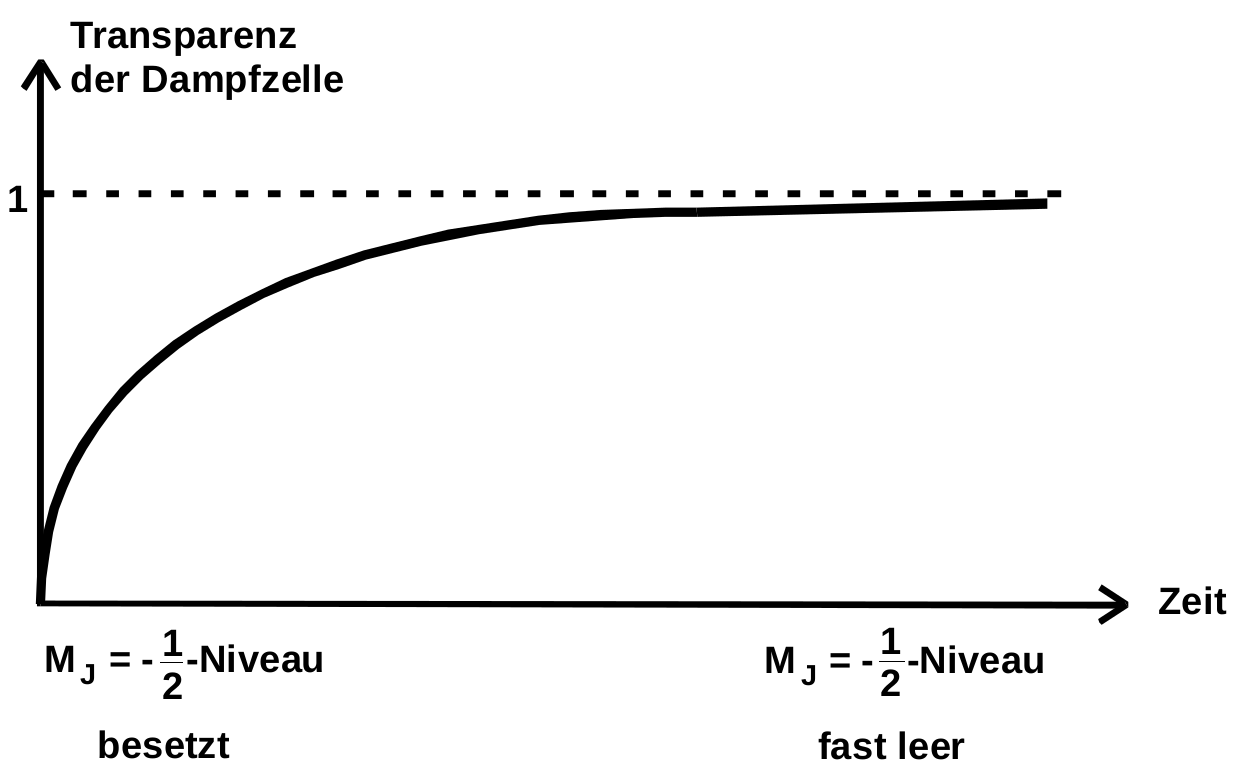
\includegraphics[height=5.5cm]{content/pictures/Transparenz.png}
  \caption{Exemplarischer Verlauf für die Transparenz der Dampfzelle in Abhängigkeit der Zeit \cite{anleitung}.}
  \label{fig:intensität}
\end{figure}

\subsection{Induzierte Emission}
\label{sec:emission}
Wie im vorherigen Abschnitt beschrieben kommt es zur Abregung des angeregten
Niveaus durch Emission von Lichtquanten. Dabei entspricht die Energie der Quanten genau der 
Energiedifferenz der beiden beteiligten Niveaus. Diese Emissionen können nicht nur
spontan auftreten, sondern auch eingeleitet werden, die so genannte induzierte Emission.
Dabei wird ein Lichtquant mit der Energie der Energiedifferenz \eqref{eqn:energiedifferenz} der beiden beteiligten 
Niveaus eingestrahlt, anschließend werden zwei Lichtquanten emittiert. Ob die spontane
oder die induzierte Emission  überwiegt ist rein von der Energiedifferenz des Übergangs abhängig.
Betrachtet man eine große Menge an Gasatomen im Temperaturgleichgewicht der Temperatur $T$, dabei befinden 
sich $N_2$ davon im angeregtem Zustand $W_2$ und $N_1$ im Grundzustand der Energie $W_1$.
Mit der Übergangswahrscheinlichkeit für die spontane Emission $A_{21}$ ergibt sich die Anzahl an 
spontanen Emissionen pro Zeiteinheit zu
\begin{equation*}
  n_\text{spon} = A_{21} N_2.
\end{equation*}
Auf Grund des Temperaturgleichgewichts, steht das Gas im Gleichgewicht mit seiner
Temperaturstrahlung, was der Strahlung eines schwarzen Körpers
\begin{equation*}
  u(\nu) = \frac{8 \pi h \nu^3}{c^2 \cdot \left(\exp{\frac{\nu h}{k_\text{B} T}} -1 \right)}
\end{equation*}
entspricht. Dabei können die Lichtquanten der Frequenz $\nu$, welche genau der Energiedifferenz zweier Niveaus entspricht
eine induzierte Emission auslösen. Dabei ergibt sich die Anzahl der induzierten Emission pro Zeiteinheit zu 
\begin{equation*}
  n_\text{ind} = B_{21} N_2 u(\nu),
\end{equation*}
mit dem Proportionalitätsfaktor der spontanen Emission $B_{21}$, der auch als Einstein-Koeffizient bezeichnet wird.
Es ist aber nicht nur die Abregung dieses Übergangs möglich sondern ebenso die Anregung, also der Übergang
vom Grundzustand in den angereten Zustand. Dabei ergibt sich die Anzahl der von Grundzustand in den angeregten Zustand
übergehenden Elektronen pro Zeiteinheit mit dem Einstein-Koeffizient für die Anregung zu
\begin{equation*}
  n_\text{an} = B_{12} N_1 u(\nu).
\end{equation*}
Da sich das System im thermischen Gleichgewicht befindet, darf sich die Besetzungszahl der Zustände nicht ändern,
es müssen sich also zu jedem Zeitpunkt die nach Formel \eqref{eqn:boltz} gegebenen Besetzungen ergeben. In Formeln ausgedrückt
ergibt sich dann
\begin{equation*}
  n_\text{spon} + n_\text{ind} = n_\text{an}.
\end{equation*}
Für den Fall nicht entarteter Niveaus gilt $B_{21} = B_{12}$, damit ergibt sich
\begin{equation}
  \label{eqn:a}
  A_{21} = \frac{8 \pi h B_{12} \nu^3}{c^3}.
\end{equation}
\begin{figure}
  \centering
  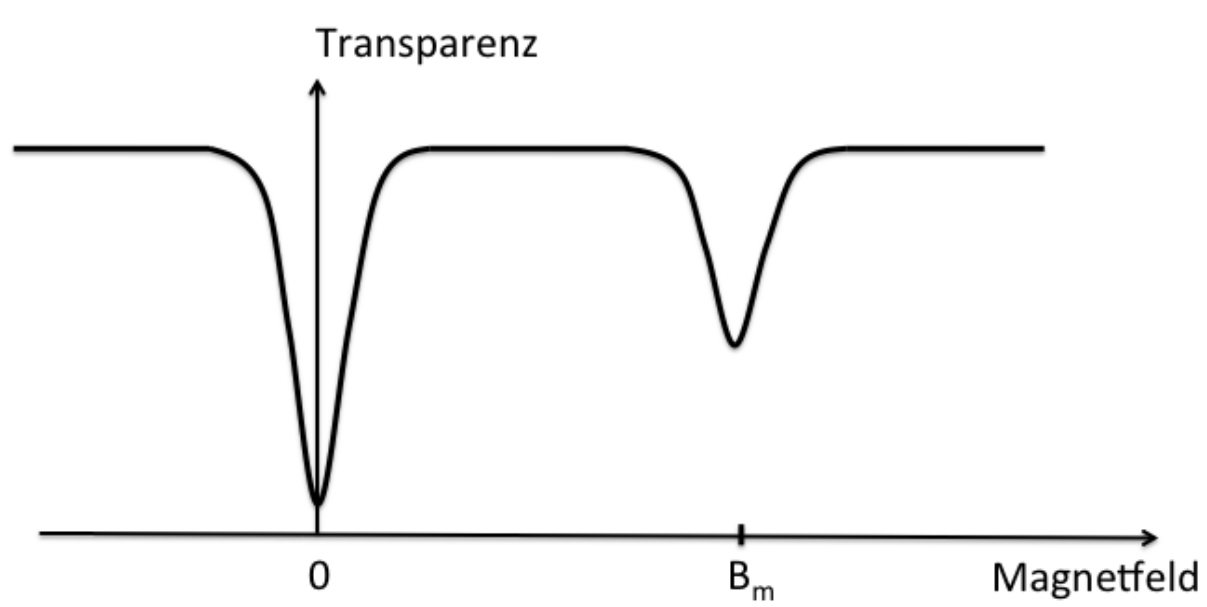
\includegraphics[height=5.5cm]{content/pictures/Resonanz.png}
  \caption{Die Transparenz der Dampfzelle in Abhängigkeit der Zeit für den Fall der Resonaz. \cite{anleitung}.}
  \label{fig:resonanz}
\end{figure}
Der Einstein-Koeffizient kann als Konstante betrachtet werden, da dieser nur von der Gestalt der 
Wellenfunktionen der beteiligten Niveaus abhängt. Da die Energiedifferenz zweier benachbarten Zeeman-Niveaus viel kleiner als
die der Übergänge zwischen Grundzustand und angeregtem Zustand ist, spielt die
spontane Emission also hier keine große Rolle. Bei der Ausmessung der Zeeman-Niveaus tritt also hauptsächlich
induzierte Emission durch die eingestrahlte Hochfrequenzstrahlung auf.
Stellt man also die eingestrahlte Hochfrequenzstrahlung durch das frequenzvariable Hochfrequenzfeld (RF) so ein,
dass genau solch eine Energiedifferenz getroffen wird, kommt es zur Resonanz.
Diese Resonanz tritt also auf, wenn die eingestrahlten Quanten genau der Energie der Zeeman-Aufspaltung nach Formel \eqref{eqn:zeeman} entsprechen.
Also 
\begin{equation*}
  h \nu = g_\text{J} \mu_\text{B} B_\text{m} \Delta M_\text{J}
\end{equation*}
entspricht. Dabei bricht dann die Transparenz der Gaszelle wieder ein, da nun das $\ce{^2 S_{\sfrac{1}{2}}}$-Niveau mit $M_\text{J}=\sfrac{-1}{2}$ wieder 
bevölkert wird. Es ergibt sich der in Abbildung \ref{fig:resonanz} skizzierte Verlauf.
Das Absinken der Transparenz um den Wert $\vec{B}=\vec{0}$ hängt damit zusammen, dass hier keine Aufspaltung in Zeeman-Niveaus vorliegt
und somit kein pumpen möglich ist. In der Realität muss man das Erdmagnetfeld beachten, denn das 
künstlich erzeugte Magnetfeld hat zwar den Wert Null, allerdings erzeugt das Erdmagnetfeld eine Aufspaltung. Die Einstellung der Nullfeld-Linie
stellt also eine gute Möglichkeit dar das Erdmagnetfeld zu bestimmen.

\begin{figure}
  \centering
  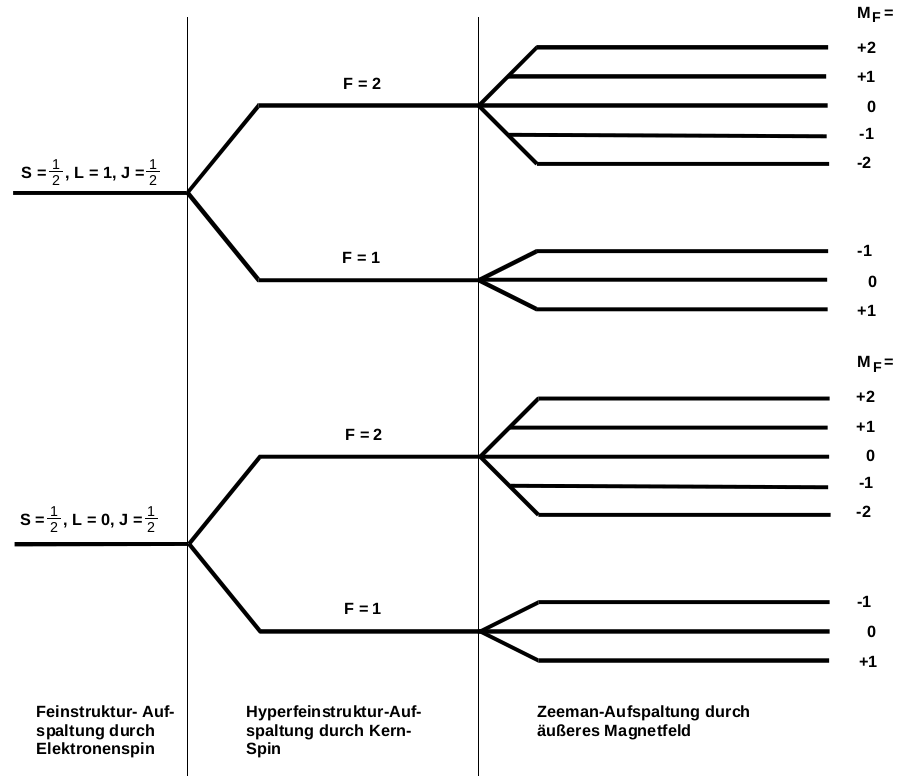
\includegraphics[height=10cm]{content/pictures/Energieniveaus2.png}
  \caption{Die Energieniveau-Aufspaltung unter Einfluss eines $\vec{B}$-Feldes und unter Beachtung des Kernspins \cite{anleitung}.}
  \label{fig:aufspaltung2}
\end{figure}
Wird nur auch der Kernspin beachtet, so ergeben sich leichte Änderungen. Das verwendete Licht wird durch eine Spektrallampe erzeugt und 
auf Grund des Doppler-Effekts ist die Energieverteilung sobreit, dass alle Übergänge der 
Hyperfeinstruktur und der Zeeman-Aufspaltung (siehe hierzu Abbildung \ref{fig:aufspaltung2}) möglich sind und nicht nur der Übergang aus
dem Grundzustand in den ersten angeregten Zustand. Da das Licht rechtszirkular-polarisiert ist
muss $M_\text{F} = +1$ erfüllt werden. Aus eben diesem Grund kann der Zustand $F = 2, M_\text{J} = 2$ keine
eingestrahlten Lichtquanten absorbieren, da kein angeregter Zustand mit $M_\text{F} = 3$ existiert. Die Besetzung dieses Zustands
kann also während des Pumpens nur zunehmen, da er durch die angeregten Zustände mit $M_\text{F} = 2, 1$ bevölkert wird, aber nicht entleer.
Nun kann aber wieder mit Hilfe von Hochfrequenzstrahlung eine induzierte Emission zwischen den Zeeman-Niveaus erzwungen werden.

Wird das äußere Magnetfeld zu stark, so wird ein Teil der inneren Kopplungen aufgehoben und 
es müssen Terme höherer Ordnung beachtet werden. Der sogenannte quadratische Zeeman-Effekt sorgt dabei, dass nicht mehr alle 
Zeeman-Übergänge gleich groß sind. Die Energiedifferenz der Zeeman-Aufspaltung ergibt sich nun nach
\begin{equation}
  \label{eqn:zeemanquadrat}
  U_\text{Z} = g_\text{F} \mu_\text{B} |\vec{B}| + g_\text{F}^2 \mu_\text{B}^2 |\vec{B}|^2 \frac{1-2 M_\text{F}}{\Delta E_\text{Hy}},
\end{equation}
mit der Hyperfeinstrukturaufspaltungsenergie $\Delta E_\text{Hy}$ zwischen $F$ und $F+1$.

\FloatBarrier
% \begin{figure}
%   \centering
%   \includegraphics[height=5.5cm]{content/pictures/Bild.png}
%   \caption{Bilduterschrift}
%   \label{fig:Bild}
% \end{figure}

% \subsection{Unterkapitel}
% \label{sec:UnterKapitel}

% \begin{equation}
% Für Formeln
%   \label{eqn:Formel}
% \end{equation}
